\documentclass[sigconf]{acmart}

% \renewcommand\footnotetextcopyrightpermission[1]{} % removes footnote with conference information in first column
\pagestyle{fancy} % removes running headers
\usepackage{booktabs} % For formal tables


\usepackage{url}
\usepackage{algorithm}
\usepackage[noend]{algpseudocode}
\algtext*{EndWhile}% Remove "end while" text
\algtext*{EndIf}% Remove "end if" text
%\usepackage{flexisym}

\setlength{\parskip}{0pt}
\setlength{\parsep}{0pt}
\setlength{\headsep}{0pt}
\setlength{\topskip}{0pt}
\setlength{\topmargin}{0pt}
\setlength{\topsep}{0pt}
\setlength{\partopsep}{0pt}
%\linespread{0.95}
\usepackage{mdwlist}

\usepackage{amsmath}
\fancyhead{}
\settopmatter{printacmref=false, printfolios=false}
% Copyright
\setcopyright{none}
% \setcopyright{acmcopyright}
% \setcopyright{acmlicensed}
% \setcopyright{rightsretained}
% \setcopyright{usgov}
% \setcopyright{usgovmixed}
% \setcopyright{cagov}
% \setcopyright{cagovmixed}

\settopmatter{printacmref=false} % Removes citation information below abstract
\begin{document}
\title{Machine Translating From English to Chinese for E-Commerce Product Categorization}\titlenote{\href{https://github.com/duongy18418/Multilingual-NLP/tree/main/Code}{https://github.com/duongy18418/Multilingual-NLP/tree/main/Code}}

% \authornote{Laboratory for Systems, Software and Semantics (LS$^3$)}
%\orcid{1234-5678-9012}

%   \streetaddress{P.O. Box 1212}
%   \city{Toronto} 
%   \state{ON} 
%   \country{Canada} 
%   \postcode{43017-6221}

\author{Kitty Duong}
\affiliation{
  \institution{University of Windsor}
  \city{Windsor}
  \country{Canada}
}
\email{duongy@uwindsor.ca}

\author{Miaomiao Zhang}
\affiliation{
  \institution{University of Windsor}
  \city{Windsor}
  \country{Canada}
}
\email{zhang3s2@uwindsor.ca}

\begin{abstract}
    In this study, we evaluate the performance of two machine translation models, NLLB-200\cite{nllb} and Google Translator\cite{baccouri}, in translating Amazon product categories\cite{amazonPromptCloud} from English to Chinese. The dataset consists of a collection of product categories extracted from the Amazon platform. We employ BLEU (Bilingual Evaluation Understudy)\cite{nltk.align.bleu_score_nltk_3.0_documentation} as the evaluation metric to compare the translations produced by the two models. Google Translator serves as the baseline system due to its widespread use and availability. The experimental results reveal the effectiveness of NLLB-200\cite{koishekenov_berard_nikoulina_2023} in capturing the nuances of the product categories, outperforming Google Translator in terms of BLEU scores. Through a comprehensive analysis of the results, we discuss the strengths and weaknesses of both translation models\cite{gauch_hwang_fick_2003}, highlighting potential areas for improvement. Our findings contribute to the understanding of machine translation performance\cite{flach_2019} in the context of e-commerce product categorization and provide insights for further research in this domain.
\end{abstract}


\keywords{Multilingual NLP, machine translation, e-commerce product categories, e-commerce translation, translation accuracy, translation evaluation, Google translator}

\maketitle
\section{Experimental Setup and Evaluation}\label{experiment}
%This section describes the experiments performed to validate our proposed work in comparison with two baselines in the context of news recommendation, user prediction, and community selection applications on a Twitter dataset.

\subsection{Dataset}
In our experiments, we use a publicly available Amazon e-commerce product category dataset \footnote{\href{https://www.kaggle.com/datasets/promptcloud/amazon-product-dataset-2020/}{https://www.kaggle.com/datasets/promptcloud/amazon-product-dataset-2020/}} collected and published by PromptCloud \cite{best_web_scraping_services_provider_company_2021}. It consists of approximately 10,000 entries based on 22 diverse main categories. Each entry of the data would include the specific and detailed subcategories under the main category, i.e., Sports Outdoors Sports Fitness Team Sports, in which "Sports Outdoors" is the main category. At the same time "Team Sports" is the second-level subcategory of the subcategory "Sports Fitness".

\subsection{Setup}
Our proposed approach consists of two phases to set up the environment for e-commerce product category translation from English to Chinese; translating the original context via a pre-trained model NLLB-200 and preparing the train data and test data. Here, we provide the implementation details and the setup of our approach in each of these phases. 

\subsubsection{Pre-trained model translation}
The translation process for converting Amazon product categories from English to Chinese using the NLLB-200 model entails preparing a standardized list of categories, setting up access to the NLLB-200 model through its API or SDK, and configuring translation parameters. Besides, we followed the tutorial from Hugging Face\cite{Hugging_Face} to use PyTorch Trainer to finetune the pre-trained model\cite{min_ross_elior_sulem_veyseh_thien_huu_nguyen_sainz_agirre_heintz_roth_2023}. We stored this model as "E-commerce\_Translation\_Model"\footnote{\href{https://huggingface.co/duongy18418/E-commerce_Translation_Model/tree/main}{https://huggingface.co/duongy18418/E-commerce\_Translation\_Model/tree/main}}, which is posted in Hugging face. Based on the configuration settings to specify the source (English) and target (Chinese) languages, we organized the product categories into batches for efficient processing, and then we sent batches to NLLB-200 for translation processing. Categories are then translated in batches, with errors and limitations managed appropriately. 

\subsubsection{Preparing training and testing data}
In the data preparation phase, we curated two distinct datasets as the training dataset $\mathbb{D}_i$ and testing dataset $\mathbb{D}_j$ , $\forall\mathbb{D}_i,\mathbb{D}_{j\neq{i}}:\mathbb{D}_i\cap\mathbb{D}_j=\varnothing$. The training data\cite{moore_lewis_2010}, derived from Google-Product, was selected due to its suitability for training machine translation models and its availability. Before training, the Google Product dataset underwent preprocessing steps, including data cleaning and tokenization, to ensure consistency and quality. Conversely, the testing data\cite{demillo_lipton_sayward_1978} consisted of Amazon e-commerce product categories, chosen to represent real-world translation scenarios relevant to our task. Preprocessing of the testing data involved similar steps to align it with the format and requirements of the translation models. Throughout this process, careful attention was paid to maintaining the integrity and representativeness of both datasets to facilitate an accurate evaluation of the translation models' performance.


\subsection{Metrics}
As for the evaluation metric, we utilized BLEU (Bilingual Evaluation Understudy)\cite{papineni_roukos_ward_zhu_2002}. BLEU is a widely used metric for evaluating the quality of machine-translated text by comparing it to one or more reference translations. It quantifies the similarity between the machine-generated translation and the reference translations based on n-gram overlap. In the context of our project, BLEU provides a standardized measure to assess the accuracy and fluency of the translated Amazon e-commerce product categories produced by the NLLB-200 and Google Translator models. A higher BLEU score\cite{mathur_baldwin_cohn_2020} indicates a closer resemblance between the generated translations and the reference translations, thus reflecting a higher quality of translation. By employing BLEU as the evaluation metric, we aim to objectively compare the performance of the two translation models across different categories of e-commerce products and provide insights into their relative strengths and weaknesses. In the result analysis part, we will display the comparison diagram based on the BLEU scores of the two models.

\subsection{Baselines}
In this report, the baseline system utilized for comparison is Google Translator. Google Translator serves as a benchmark against which the performance of the NLLB-200 model in translating Amazon e-commerce product categories from English to Chinese is evaluated. Google Translator\cite{sutrisno_2020} is chosen as the baseline due to its widespread use and availability as a popular machine translation tool. By comparing the translations generated by NLLB-200 with those produced by Google Translator, we can assess the relative effectiveness and accuracy of the NLLB-200 model in capturing the nuances of the product categories. The comparison with Google Translator provides a practical reference point for evaluating the performance of NLLB-200 and gaining insights into its strengths and limitations. Additionally, the baseline comparison helps contextualize the results obtained from NLLB-200, offering valuable benchmarks for assessing the progress and advancements in machine translation technology.

\subsection{Evaluation results}
In the result section of this report, we will provide a comprehensive analysis of the performance of both the baseline model (Google Translator) and the proposed model (E-commerce-Translation-Model) based on the BLEU scores obtained. The result analysis is conducted from perspectives of BLEU scores and runtime comparison.

\subsubsection{BLEU scores}
The BLEU scores obtained for the E-commerce-Translation-Model demonstrate a slightly higher and more consistent performance than the baseline model, Google Translator. Across various categories of e-commerce products, the E-commerce-Translation-Model consistently yielded BLEU scores that were marginally superior to those of the baseline model. This suggests that the proposed model may better capture the nuances of product descriptions and translate them accurately from English to Chinese. Despite the modest improvements observed in BLEU scores\cite{mathur_baldwin_cohn_2020}, it's important to note that both models' translations fall significantly below the ideal score of 1, indicating that there is still room for improvement in terms of translation quality.
\begin{figure}[t]
\centering
\captionsetup{justification=centering}
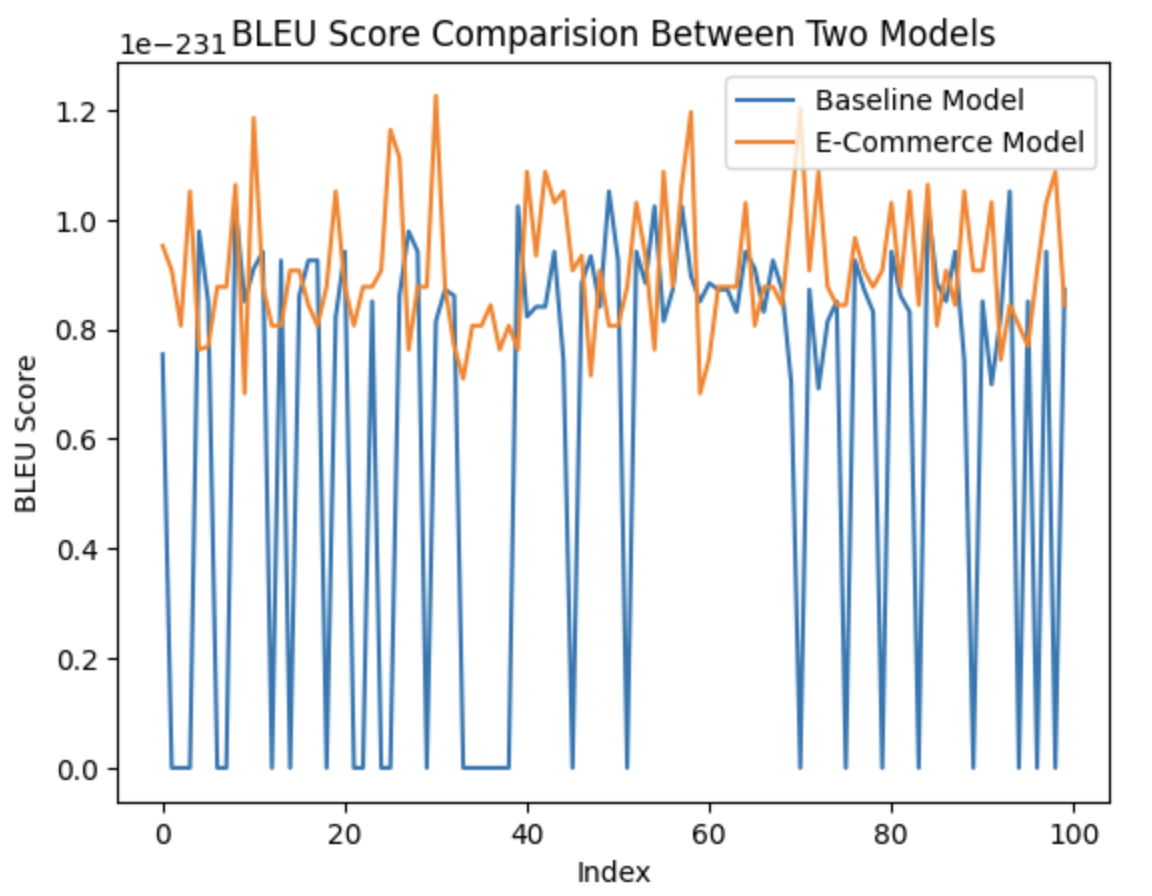
\includegraphics[width=1.05\columnwidth]{./Images/res.png}
\caption{Comparative performance on Baseline model and E-commerce model.}
\end{figure}

\subsubsection{Runtime comparison}
In terms of runtime, the proposed model E-commerce-Translation-Model exhibited a substantially longer processing time compared to the baseline model. The E-commerce-Translation Model took approximately 287.72 seconds to complete the translation task, whereas the baseline model only required 22.18 seconds. This significant disparity in runtime raises concerns about the scalability and efficiency of the E-commerce-Translation-Model, particularly in real-world applications where speed and responsiveness are critical factors. Further investigation is warranted to identify the factors contributing to the increased computational complexity\cite{goldreich_2008} of the E-commerce-Translation-Model and explore strategies for optimizing its performance without compromising translation quality.





\bibliographystyle{ACM-Reference-Format}
\bibliography{bibliography.bib} 

\end{document}